\subsection{Begriff}

Die Polarisation ist festgelegt durch die Schwingungsebene des elektrischen Feldes des Lichtes. Natürliches Licht ist unpolarisiert, das heißt es enthält Licht aller Polarisationsrichtungen, also es enthält Wellen aller Schwingungsebenen.

Mit Schwingungsebene meint man die Ausrichtung der Ebene, in der sich die Schwingungsvektoren des elektrischen Feldes befinden. Diese stehen immer Senkrecht auf dem Vektor der Ausbreitungsrichtung, aber es gibt trotzdem unendlich viele Möglichkeiten für die Ausrichtung des Feldes. Siehe Abbildung \ref{fig:emwelle} auf Seite \pageref{fig:emwelle}: die blauen Vektorpfeile sind die Schwingungsvektoren des elektrischen Feldes.

\subsection{Polarisationsfilter}

Ein Polarisationsfilter lässt nur Licht, welches in eine bestimmte Richtung polarisiert ist, zu 100\% durch. 

Wenn Licht bereits polarisiert ist, also nur noch eine Schwingungsebene existiert, wird es vom Filter 100\% durchgelassen, wenn er sich in der sogenannten Transmissionsrichtung befindet. Steht er 90\degree{} zur Transmissionsrichtung, wird das Licht zu 100\% abgeschirmt, also nichts durchgelassen.

Das Malus'sche Gesetzt gibt die resultierende Intensität des Lichtes nach dem Filter in Abhängigkeit von der Anfangsintensität $I_1$ und dem Winkel des Filters zur Transmissionsrichtung $\Theta$ (sprich: \glqq groß Theta\grqq ) an:

\begin{align}
\begin{split}
	I_2 = I_1 \cdot cos^2(\Theta)
\end{split}
\end{align}

\subsection{Brewster-Winkel}

\begin{figure}[!h]
	\centering
	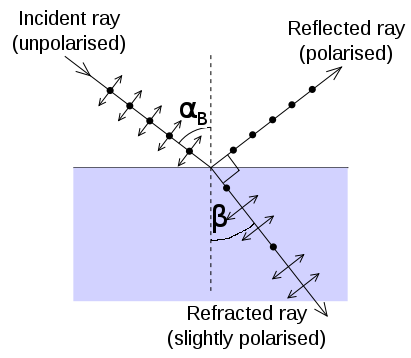
\includegraphics[width=0.7\textwidth]{brewster_2}
	\caption{Illustration des Brewster-Winkels}
	\label{fig:brewster}
\end{figure}

Licht kann auch durch Reflexion polarisiert werden. Aber nur, wenn das Licht im Brewster-Winkel auf die Reflexionsebene auftrifft, wird der reflektierte Strahl vollständig polarisiert. Nach der Polarisation steht die Ebene das elektrischen Feldes parallel zur Reflexionsebene.

Die Bedingung für vollständige Polarisation: Der Winkel zwischen reflektiertem und gebrochenem Strahl muss $90\degree$ sein. Dies ist die Definition des Brewster Winkels.

Man kann ihn sich mit der Grafik \ref{fig:brewster}\endnote{\glqq Brewsters-angle\grqq{} by Pajs - Eigen werk. Licensed under Publiek domein via Wikimedia Commons - \url{https://commons.wikimedia.org/wiki/File:Brewsters-angle.svg} modifiziert von Till Blaha} herleiten:

Mit dem Brechungsgesetz (Siehe \gleichungsreferenz{eq:brechungsgesetz}) und in der Luft: $n_1 \approx 1$, gilt:

\begin{align}
\begin{split}
	\beta &= 90\degree - \alpha_B \\
	\frac{\sin{\alpha_B}}{\sin{90\degree - \alpha}} &= \frac{n_2}{n_1} \\
	\frac{\sin{\alpha_B}}{\cos{\alpha_B}} &= n_2 \\
	\tan{\alpha_B} &= n_2 \\
	\alpha_B &= \arctan{n_2}
\end{split}
\end{align}